\documentclass{beamer}
%% Possible paper sizes: a0, a0b, a1, a2, a3, a4.
%% Possible orientations: portrait, landscape
%% Font sizes can be changed using the scale option.
\usepackage[size=a0,orientation=landscape,scale=0.7]{beamerposter}
\usetheme{LLT-poster}
\usecolortheme{ComingClean}
%\usecolortheme{Entrepreneur}
% \usecolortheme{ConspiciousCreep}  %% VERY garish.

\usepackage{polyglossia}   %% загружает пакет многоязыковой вёрстки
\setdefaultlanguage{russian}  %% устанавливает главный язык документа
%\setdefaultlanguage[babelshorthands=true]{russian}  %% вместо предыдущей строки; доступны команды из пакета babel для русского языка
\setotherlanguage{english} %% объявляет второй язык документа
\defaultfontfeatures{Ligatures={TeX},Renderer=Basic}  %% свойства шрифтов по умолчанию. Для XeTeX опцию Renderer=Basic можно не указывать, она необходима для LuaTeX
%\setmainfont[Ligatures={TeX,Historic}]{CMU Serif} %% задаёт основной шрифт документа
%\setsansfont{CMU Sans Serif}         
%\setsansfont{Linux Libertine O}                               %% задаёт шрифт без засечек
%\setmonofont{CMU Typewriter Text}               %% задаёт моноширинный шрифт
\usepackage{libertine}
\usepackage[scaled=0.92]{inconsolata}
\usepackage[libertine]{newtxmath}
\usepackage{wrapfig}
\usepackage{lipsum}
\newfontfamily{\cyrillicfonttt}{Courier New}

\author[]{Оля Гнилова}
\title{Прогнозирование временных рядов с помощью модели состояние-наблюдение}
\institute{Высшая школа экономики, 2017}


\begin{document}
\begin{frame}[fragile]\centering

\begin{columns}[T]
\begin{column}{.32\textwidth}

\begin{columns}[T]
\begin{column}{.49\textwidth}

\begin{block}{ Моделирование ошибкой}



\[
y_t = \varepsilon_t, \varepsilon_t \sim \mathcal{N}(0, \sigma^2_\varepsilon)
\]

\begin{figure}[htb]
  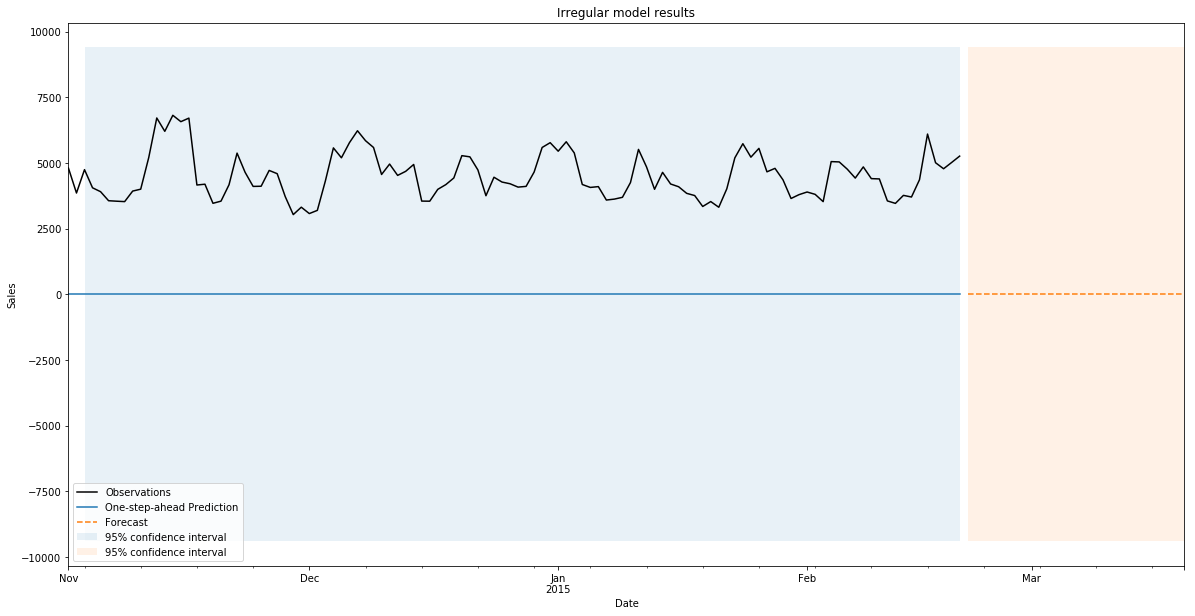
\includegraphics[width=0.97\linewidth]{1_irregular.png}
\end{figure}
\begin{figure}[htb]
  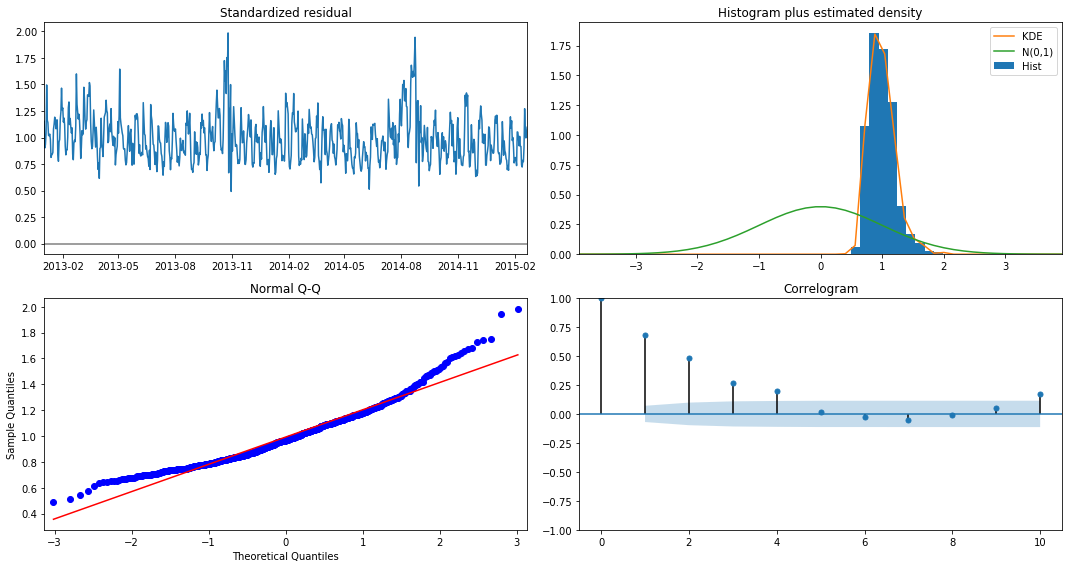
\includegraphics[width=0.97\linewidth]{1_irregular_res.png}
\end{figure}
\end{block}
\end{column}

\begin{column}{.49\textwidth}

\begin{block}{Моделирование константой}


\[
y_{t} = \mu + \varepsilon_{t}, \varepsilon_{t} \sim \mathcal{N}(0, \sigma^{2}_{\varepsilon})
\]

\begin{figure}[htb]
  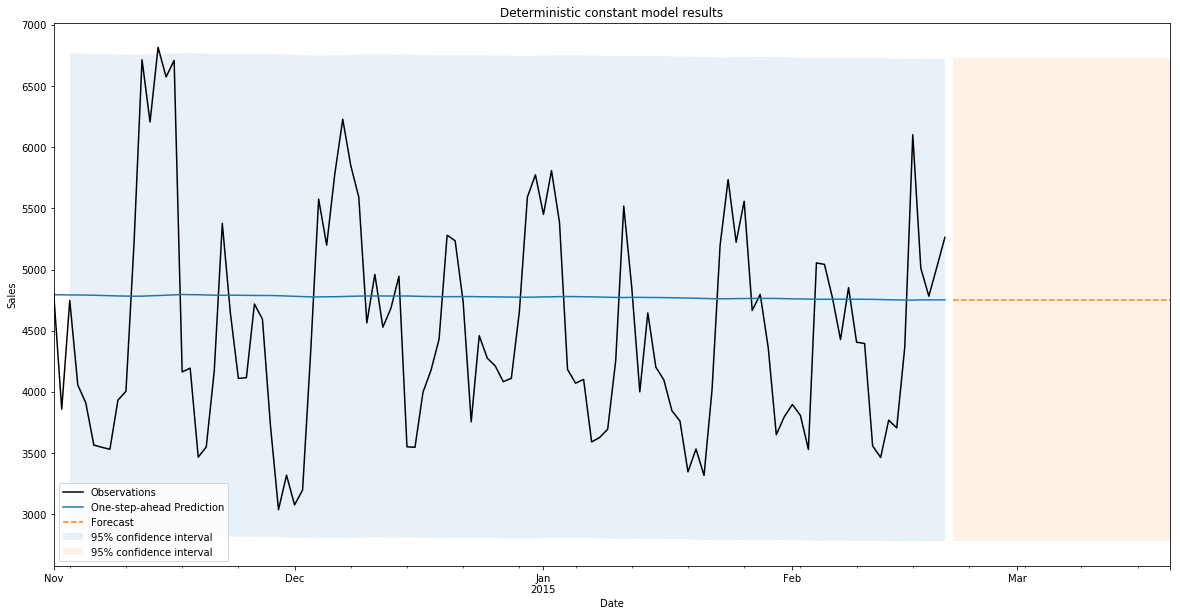
\includegraphics[width=0.97\linewidth]{2_detconst.png}
\end{figure}
\begin{figure}[htb]
  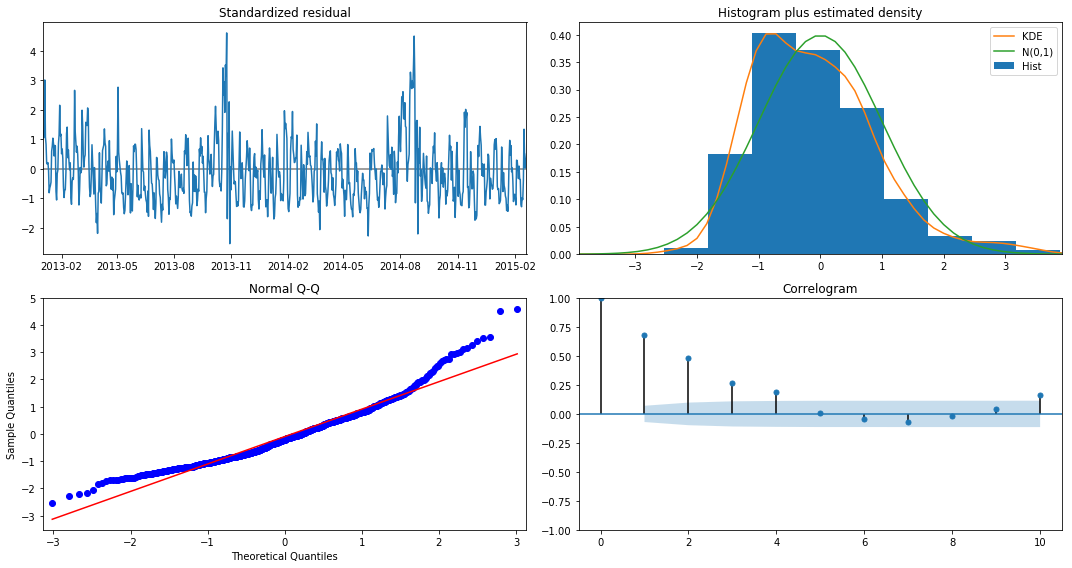
\includegraphics[width=0.97\linewidth]{2_detconst_res.png}
\end{figure}
\end{block}
\end{column}
\end{columns}

\begin{block}{Модель локального уровня}

\vspace{-0.25cm}

\begin{figure}[htb]
\minipage{0.49\textwidth}
\begin{gather*}
y_{t} = \mu_{t} + \varepsilon_{t}, \varepsilon_{t} \sim \mathcal{N}(0, \sigma^2_\varepsilon) 
\\
\mu_{t+1} = \mu_{t} + \eta_{t}, \eta_{t} \sim \mathcal{N}(0, \sigma_{\eta}^{2}) 
\\
\mu_1 \sim \mathcal{N}(a_{1}, P_{1})
\end{gather*}
\endminipage \hfill
\minipage{0.49\textwidth}
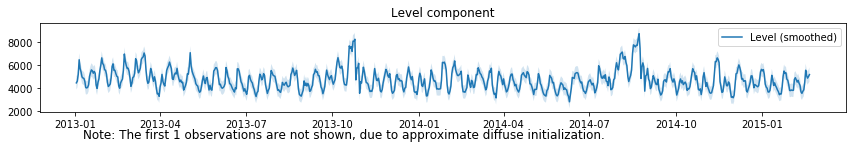
\includegraphics[width=0.99\linewidth]{3_level_small.png}
\endminipage\hfill
\end{figure}

\begin{figure}[htb]
\minipage{0.49\textwidth}
  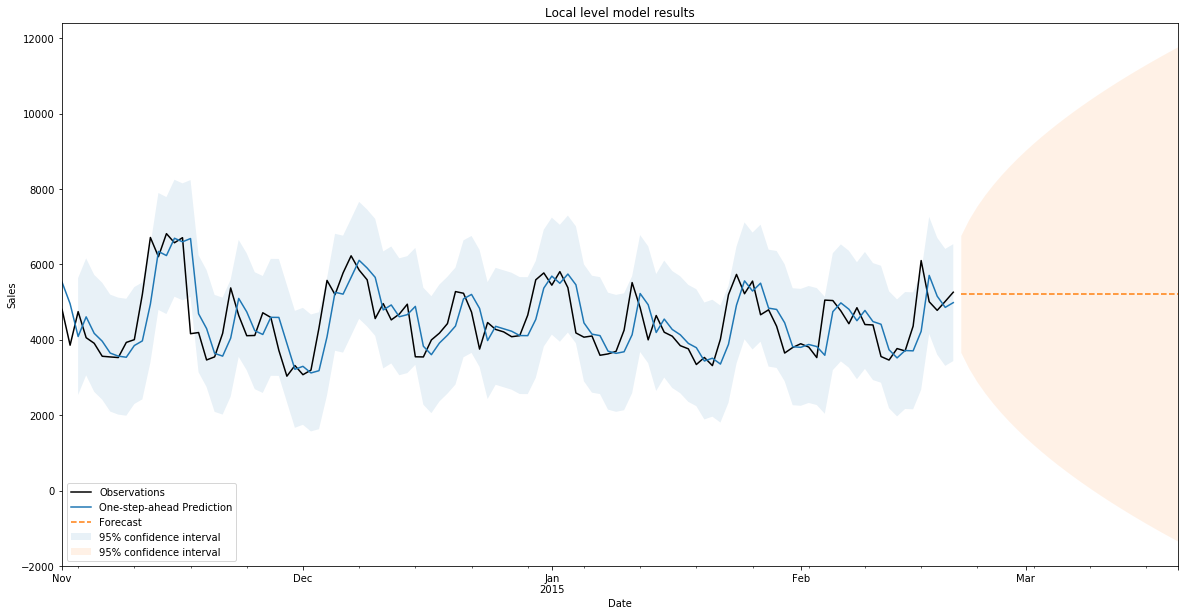
\includegraphics[width=0.99\linewidth]{3_loclev.png}
\endminipage\hfill
\minipage{0.49\textwidth}
  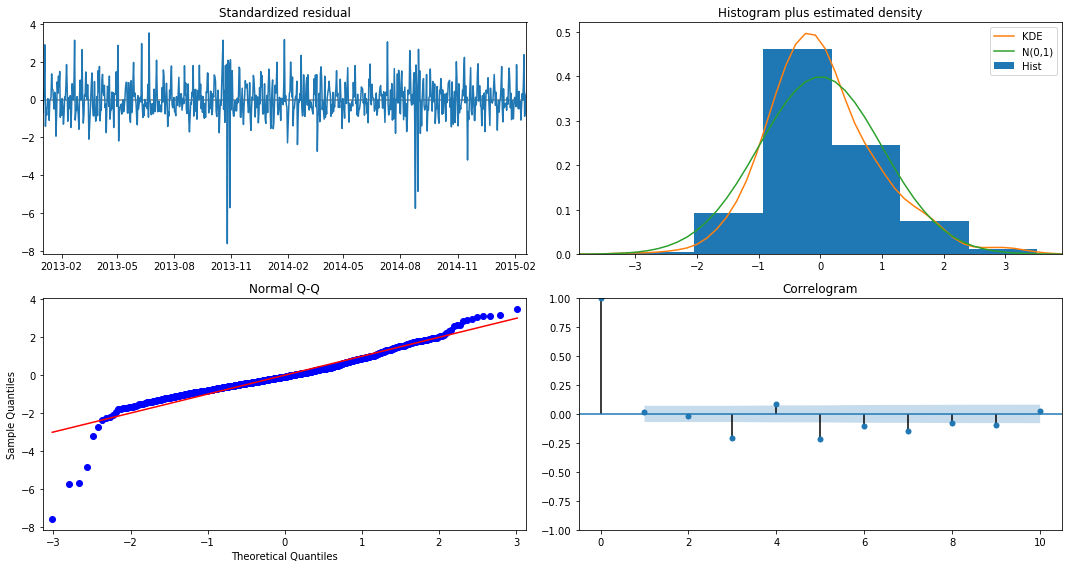
\includegraphics[width=0.99\linewidth]{3_loclev_res.png}
\endminipage\hfill
\end{figure}
\end{block}

\begin{block}{Случайное блуждание}

\vspace{-0.25cm}

\begin{figure}[htb]
\minipage{0.49\textwidth}
\begin{gather*}
y_t = \mu_t
\\
\mu_t = \mu_{t-1} + \eta_t , \eta_t \sim \mathcal{N}(0, \sigma_\eta^2)
\end{gather*}
\endminipage \hfill
\minipage{0.49\textwidth}
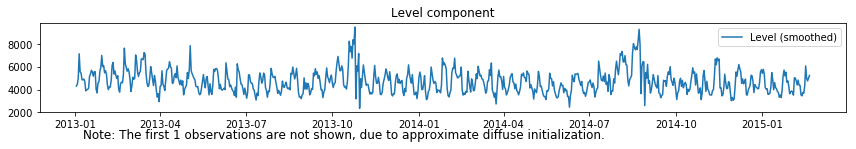
\includegraphics[width=0.99\linewidth]{4_level_small.png}
\endminipage\hfill
\end{figure}

\begin{figure}[htb]
\minipage{0.49\textwidth}
  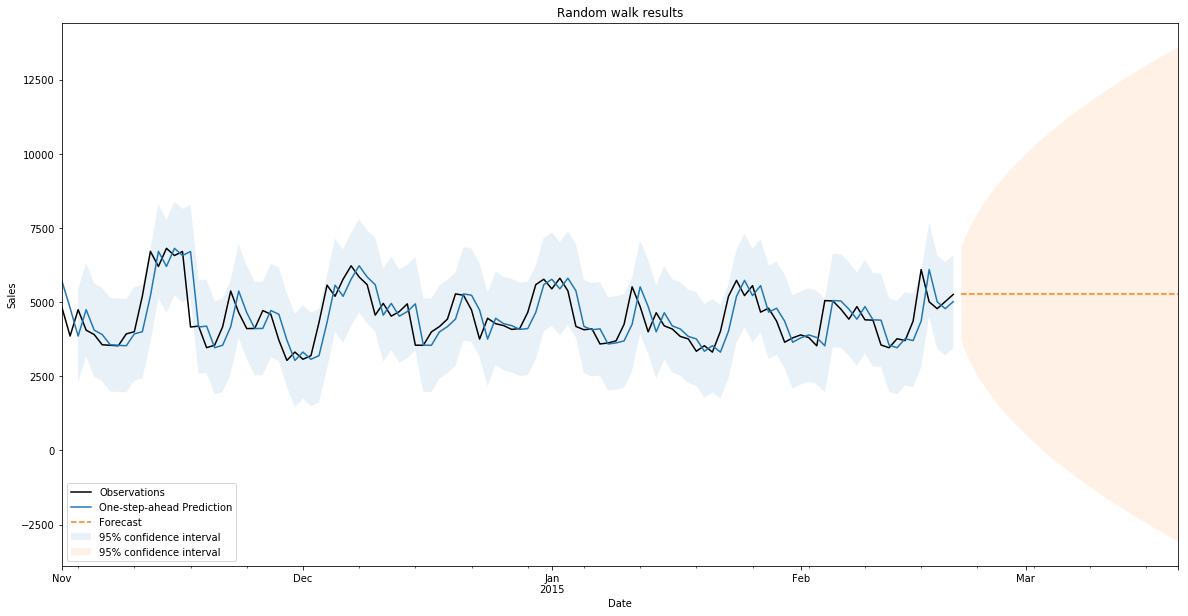
\includegraphics[width=0.99\linewidth]{4_randwalk.png}
\endminipage\hfill
\minipage{0.49\textwidth}
  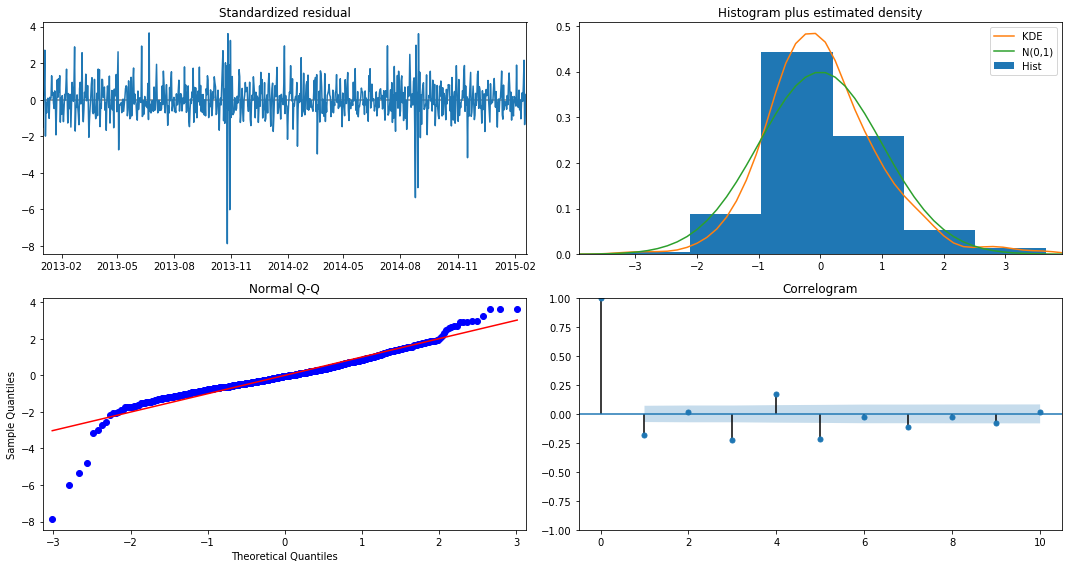
\includegraphics[width=0.99\linewidth]{4_randwalk_res.png}
\endminipage\hfill
\end{figure}
\end{block}

\begin{block}{Постоянный тренд}

\vspace{-0.5cm}

\[
y_t = \mu_t + \varepsilon_t, \varepsilon_t \sim \mathcal{N}(0, \sigma^2_\varepsilon)
\]
\[
\mu_t = \mu_{t-1} + \beta
\]

\begin{figure}[htb]
\minipage{0.49\textwidth}
  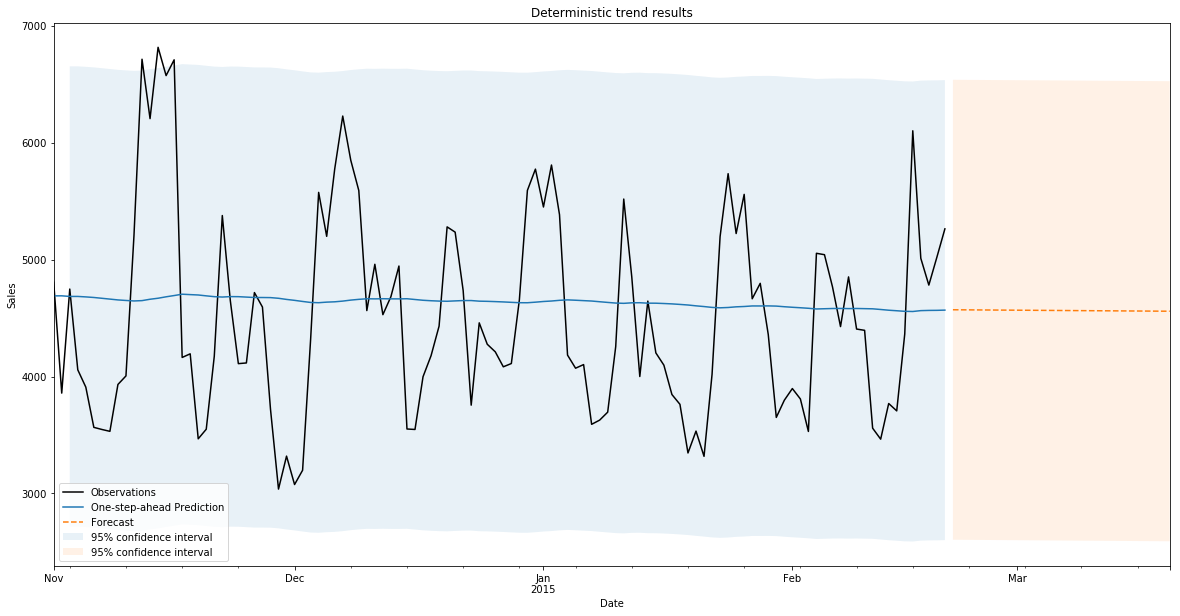
\includegraphics[width=0.99\linewidth]{5_dettrend.png}
\endminipage\hfill
\minipage{0.49\textwidth}
  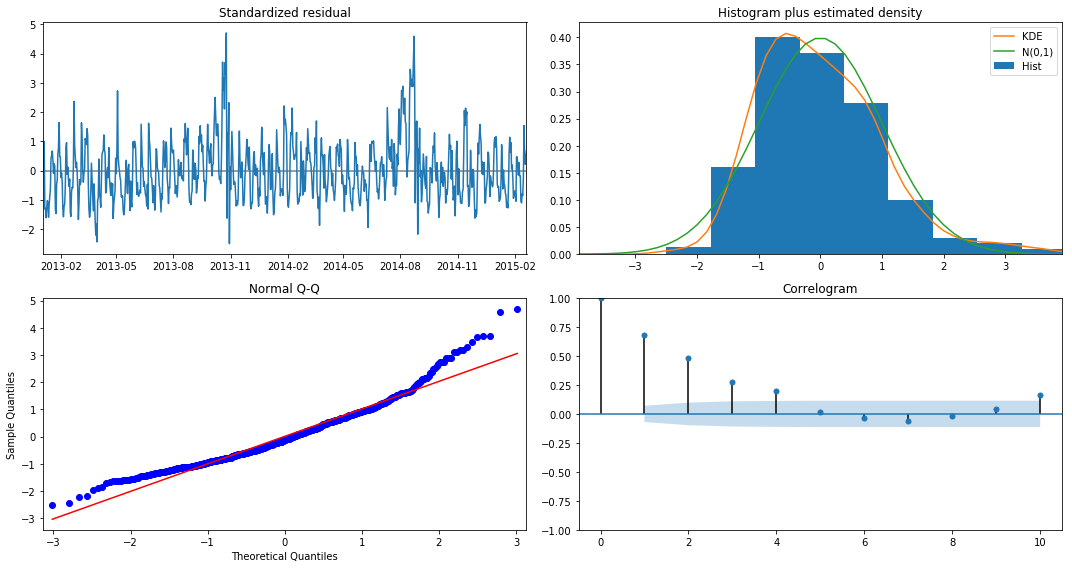
\includegraphics[width=0.99\linewidth]{5_dettrend_res.png}
\endminipage\hfill
\end{figure}

\vspace{-0.25cm}

\begin{figure}[htb]
\minipage{0.49\textwidth}
  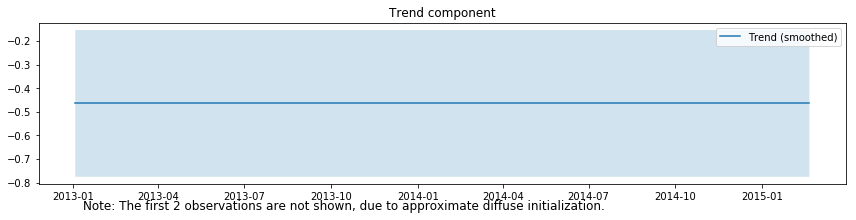
\includegraphics[width=0.99\linewidth]{5_trend.png}
\endminipage\hfill
\minipage{0.49\textwidth}
  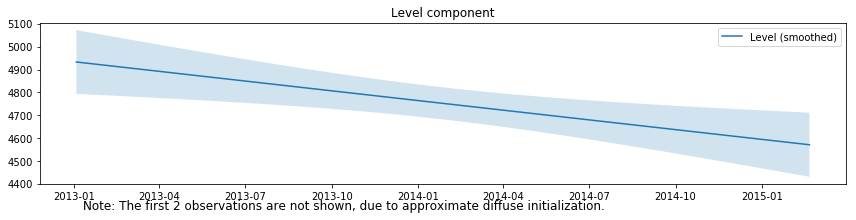
\includegraphics[width=0.99\linewidth]{5_level.png}
\endminipage\hfill
\end{figure}
\end{block}

\end{column}

\begin{column}{.32\textwidth}

\begin{block}{Локальный линейный постоянный тренд}

\vspace{-0.25cm}

\[
y_t = \mu_t + \varepsilon_t, \varepsilon_t \sim \mathcal{N}(0, \sigma^2_\varepsilon)
\]
\[
\mu_t = \mu_{t-1} + \beta + \eta_t, \eta_t \sim \mathcal{N}(0, \sigma^2_\eta)
\]

\begin{figure}[htb]
\minipage{0.49\textwidth}
  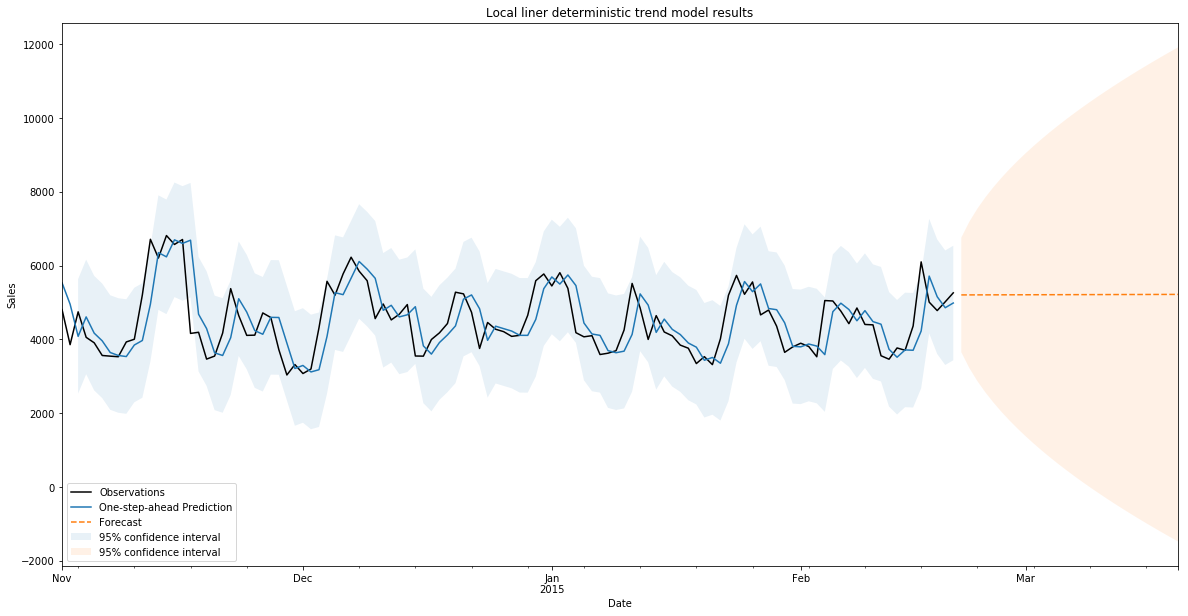
\includegraphics[width=0.99\linewidth]{6_lldtrend.png}
\endminipage\hfill
\minipage{0.49\textwidth}
  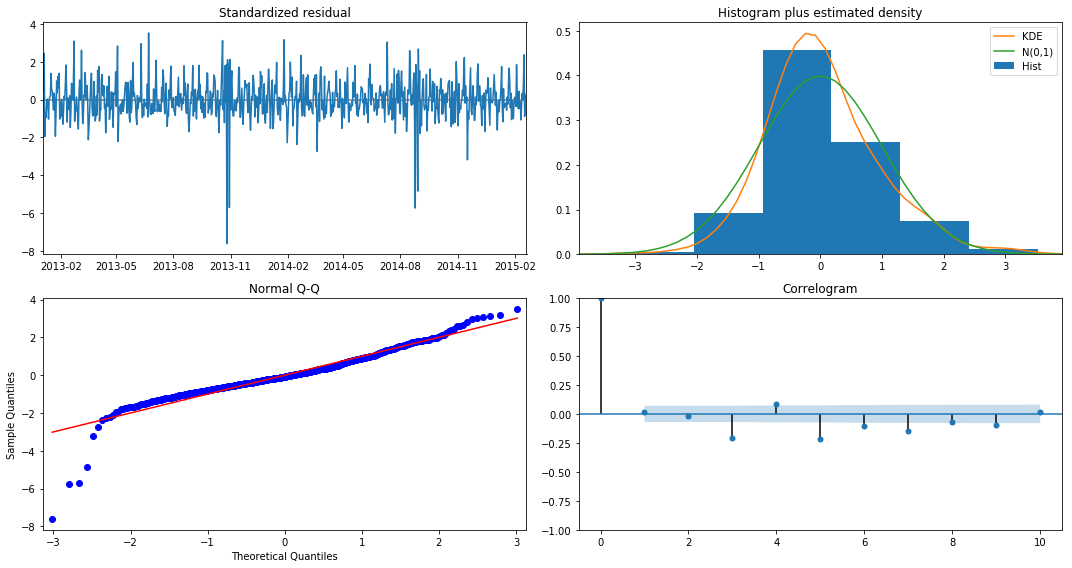
\includegraphics[width=0.99\linewidth]{6_lldtrend_res.png}
\endminipage\hfill
\end{figure}

\begin{figure}[htb]
\minipage{0.49\textwidth}
  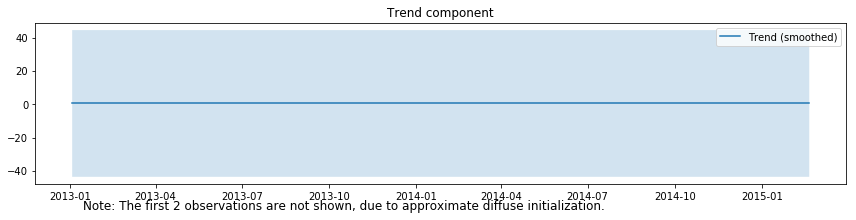
\includegraphics[width=0.99\linewidth]{6_trend.png}
\endminipage\hfill
\minipage{0.49\textwidth}
  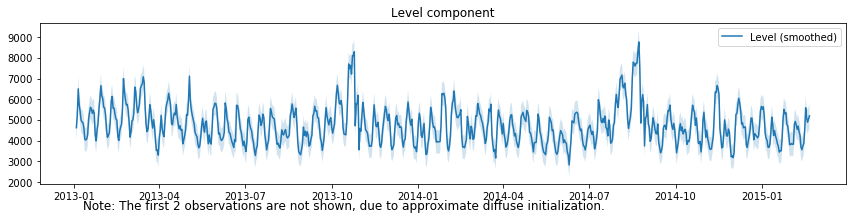
\includegraphics[width=0.99\linewidth]{6_level.png}
\endminipage\hfill
\end{figure}
\end{block}

\begin{block}{Случайное блуждание со смещением}

\vspace{-0.25cm}

\[
y_t = \mu_t 
\]
\[
\mu_t = \mu_{t-1} + \beta + \eta_t, \eta_t \sim \mathcal{N} (0, \sigma_\eta^2)
\]

\begin{figure}[htb]
\minipage{0.49\textwidth}
  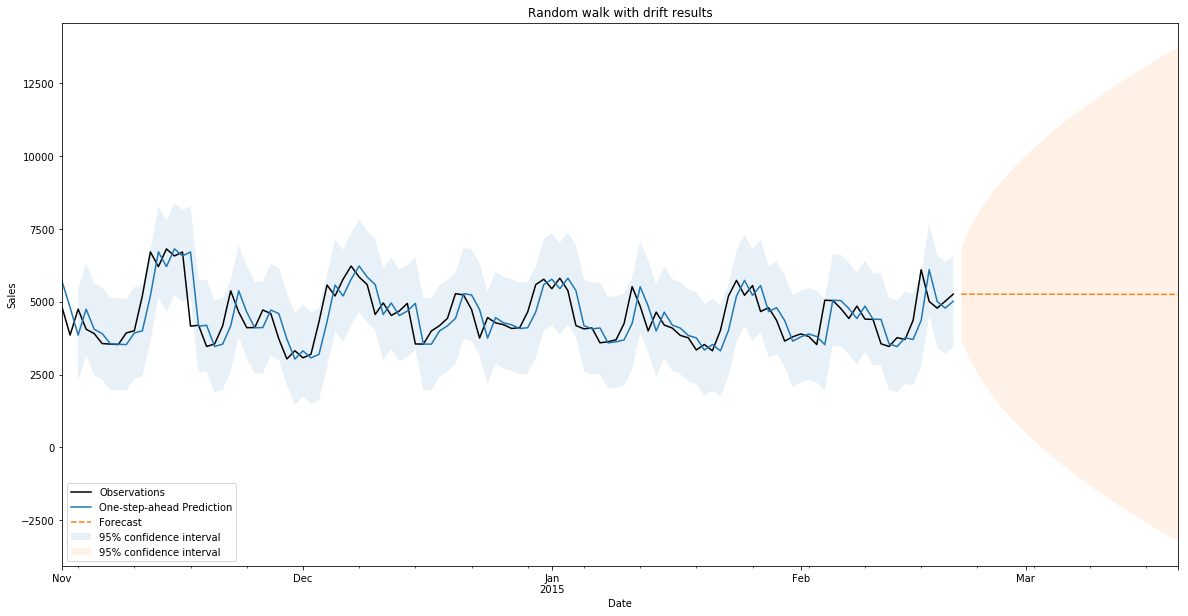
\includegraphics[width=0.99\linewidth]{7_randwalkwdrift.png}
\endminipage\hfill
\minipage{0.49\textwidth}
  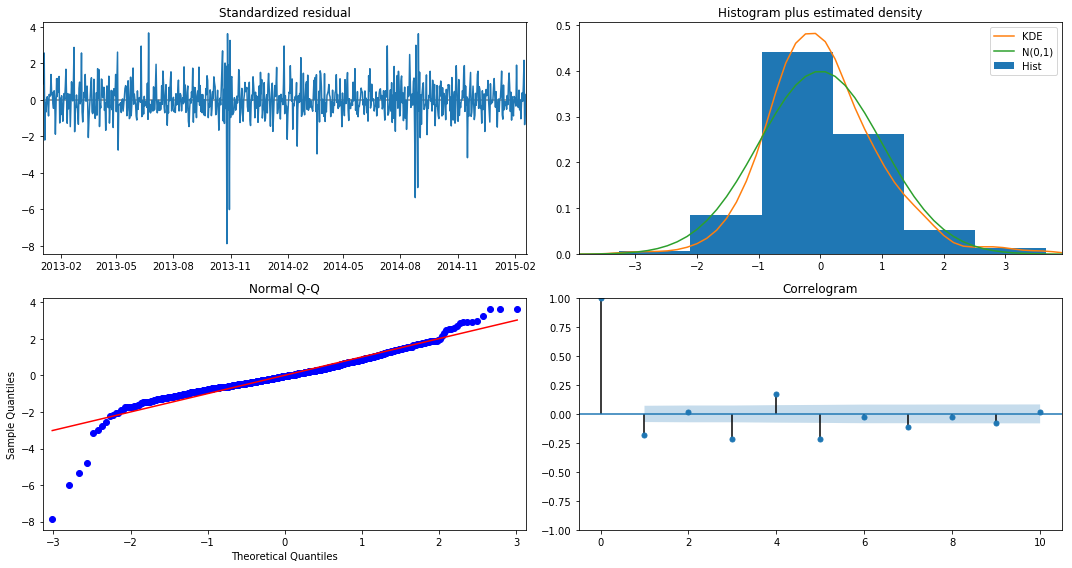
\includegraphics[width=0.99\linewidth]{7_randwalkwdrift_res.png}
\endminipage\hfill
\end{figure}

\begin{figure}[htb]
\minipage{0.49\textwidth}
  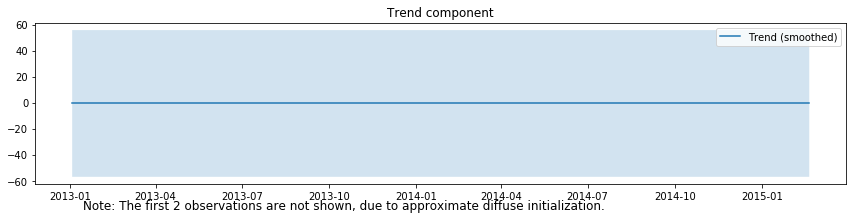
\includegraphics[width=0.99\linewidth]{7_trend.png}
\endminipage\hfill
\minipage{0.49\textwidth}
  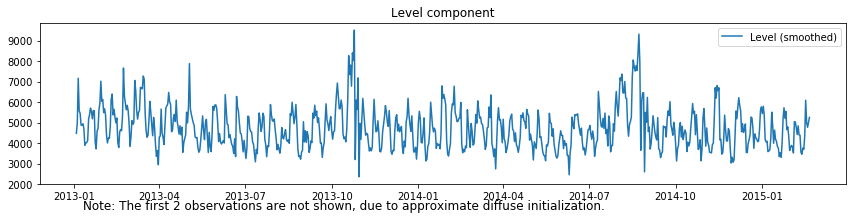
\includegraphics[width=0.99\linewidth]{7_level.png}
\endminipage\hfill
\end{figure}
\end{block}

\begin{columns}[T]
\begin{column}{.49\textwidth}

\begin{block}{Локальный линейный тренд}

\vspace{-0.25cm}

\[
y_t = \mu_t + \varepsilon_t, \varepsilon_t \sim \mathcal{N}(0, \sigma^2_\varepsilon)
\]
\[
\mu_t = \mu_{t-1} + \beta_{t-1} + \eta_t, \eta_t \sim \mathcal{N}(0, \sigma^2_\eta)
\]
\[
\beta_t = \beta_{t-1} + \zeta_t, \zeta_t \sim \mathcal{N}(0, \sigma_\zeta^2)
\]

\begin{figure}[htb]
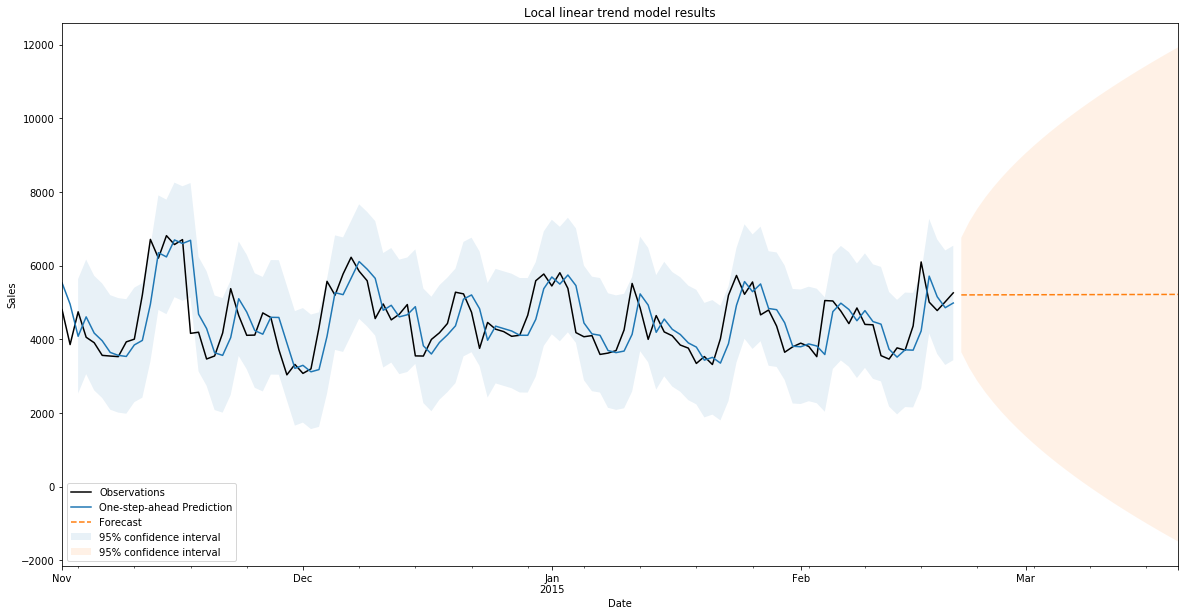
\includegraphics[width=0.97\linewidth]{8_loclintr.png}
\end{figure}

\begin{figure}[htb]
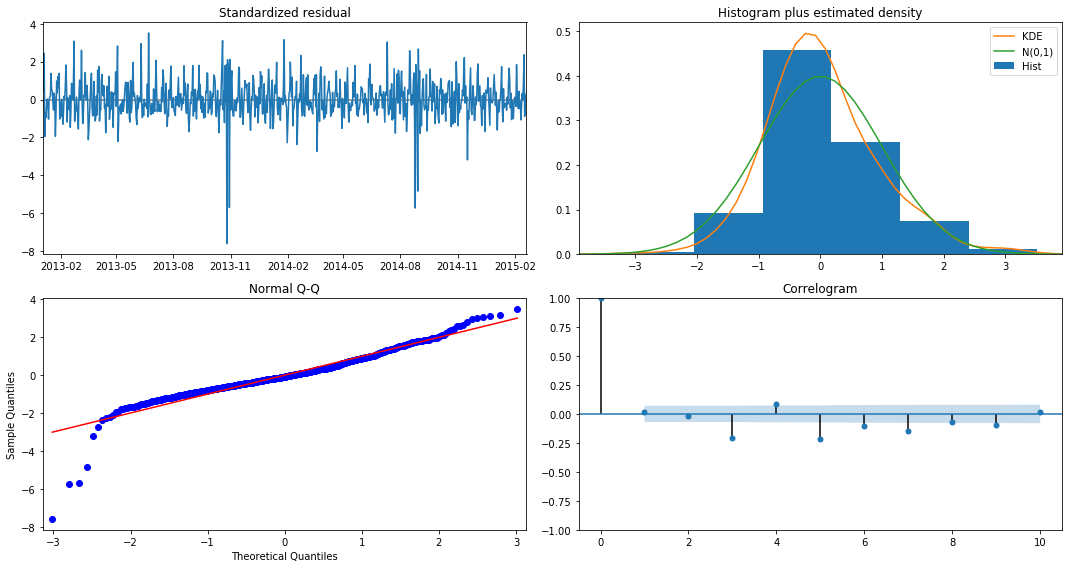
\includegraphics[width=0.97\linewidth]{8_loclintr_res.png}
\end{figure}

\begin{figure}[htb]
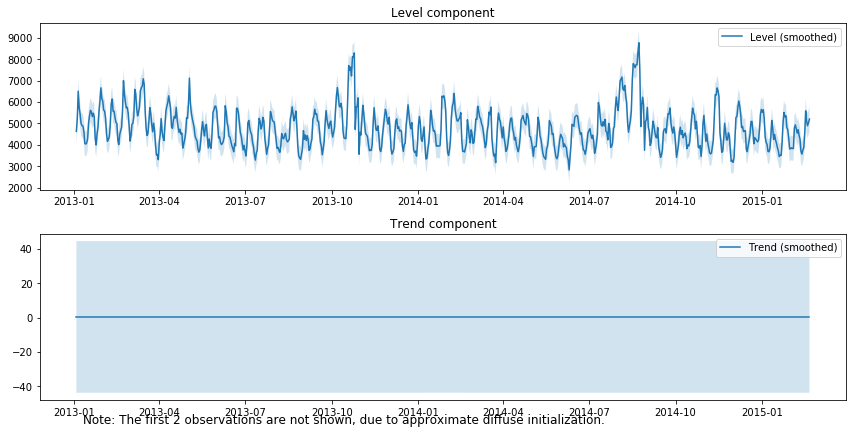
\includegraphics[width=0.97\linewidth]{8_loclintr_dec.png}
\end{figure}

\end{block}
\end{column}

\begin{column}{.5\textwidth}
\begin{block}{Сглаженный тренд}

\vspace{-0.25cm}

\[
y_t = \mu_t + \varepsilon_t, \varepsilon_t \sim \mathcal{N}(0, \sigma^2_\varepsilon)
\]
\[
\mu_t = \mu_{t-1} + \beta_{t-1}
\]
\[
\beta_t = \beta_{t-1} + \zeta_t, \zeta_t \sim \mathcal{N}(0, \sigma_\zeta^2)
\]

\begin{figure}[htb]
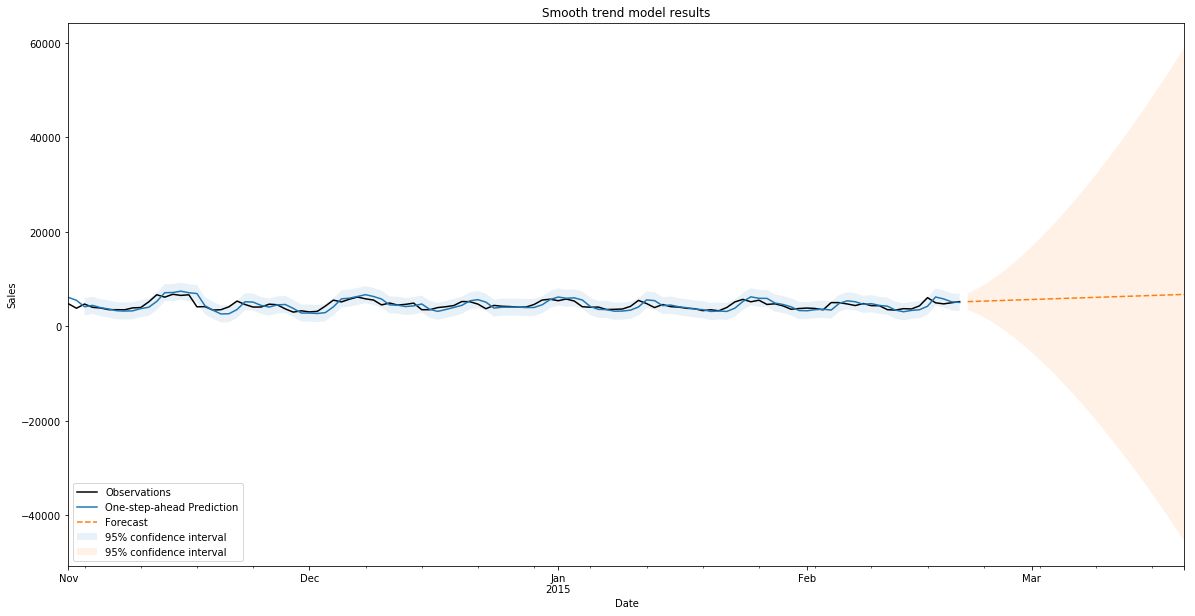
\includegraphics[width=0.97\linewidth]{9_smtrend.png}
\end{figure}

\vspace{-0.13cm}

\begin{figure}[htb]
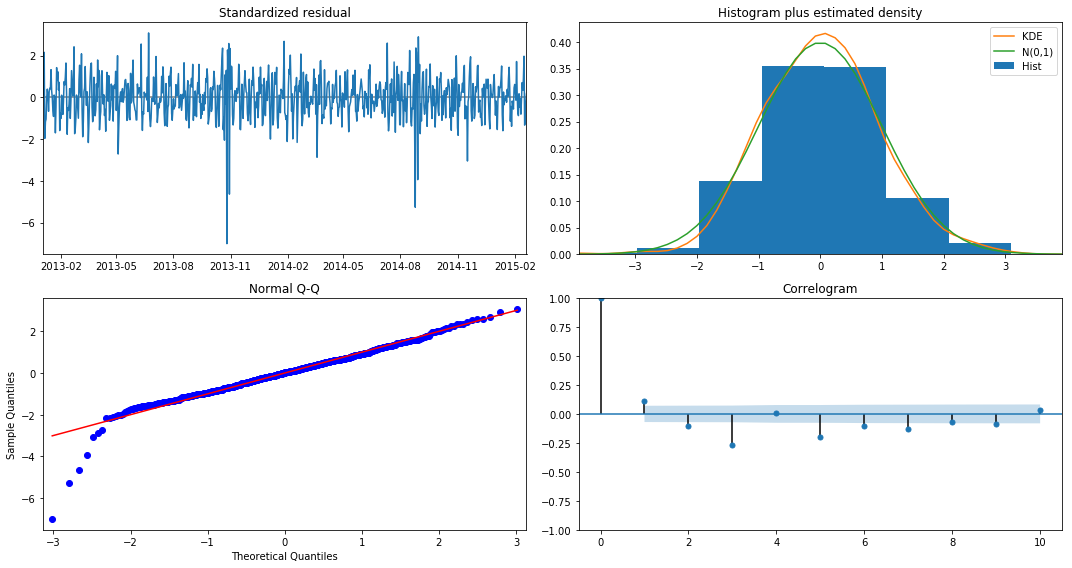
\includegraphics[width=0.97\linewidth]{9_smtrend_res.png}
\end{figure}

\vspace{-0.14cm}

\begin{figure}[htb]
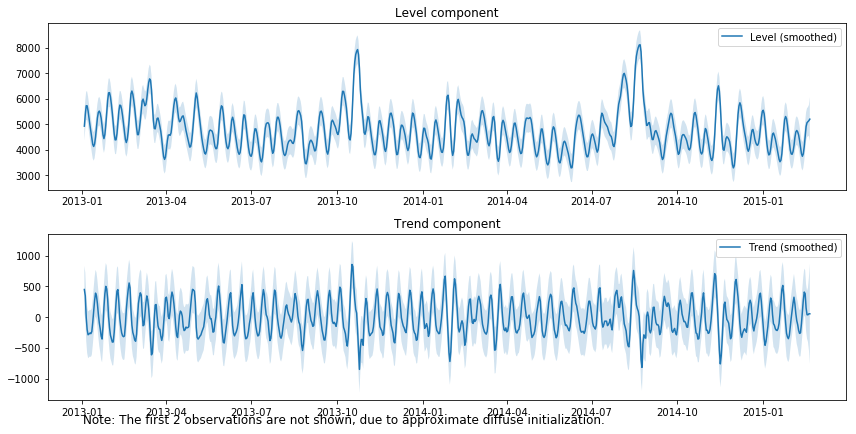
\includegraphics[width=0.97\linewidth]{9_smtrend_dec.png}
\end{figure}

\end{block}
\end{column}

\end{columns}
\end{column}

\begin{column}{.32\textwidth}

\begin{block}{Случайный тренд}

\begin{figure}[htb]
\minipage{0.49\textwidth}
\begin{gather*}
y_t = \mu_t
\\
\mu_t = \mu_{t-1} + \beta_{t-1}
\\
\beta_t = \beta_{t-1} + \zeta_t, \zeta_t \sim \mathcal{N}(0, \sigma_\zeta^2)
\end{gather*}
\endminipage \hfill
\minipage{0.49\textwidth}
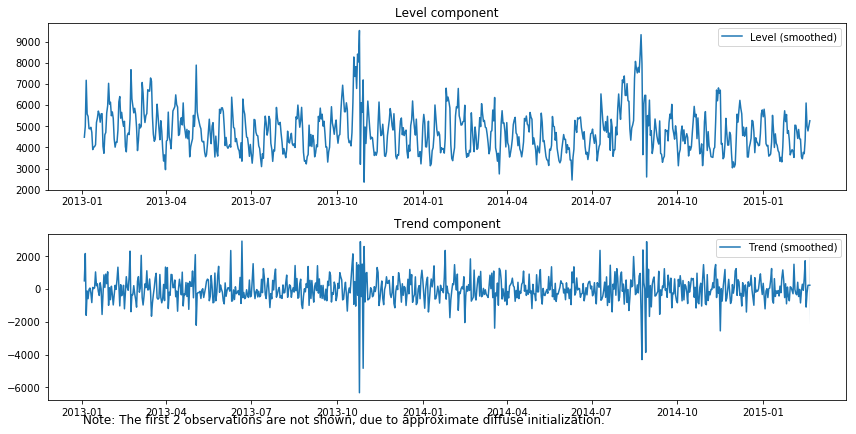
\includegraphics[width=0.99\linewidth]{10_randtrend_dec.png}
\endminipage\hfill
\end{figure}

\begin{figure}[htb]
\minipage{0.49\textwidth}
  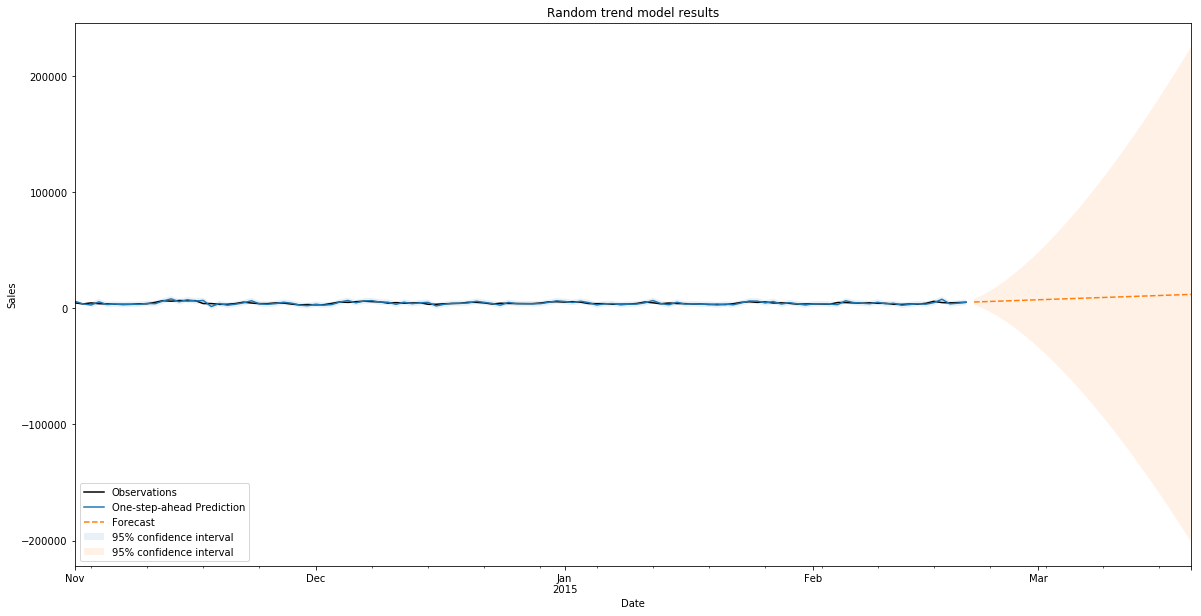
\includegraphics[width=0.99\linewidth]{10_randtrend.png}
\endminipage\hfill
\minipage{0.49\textwidth}
  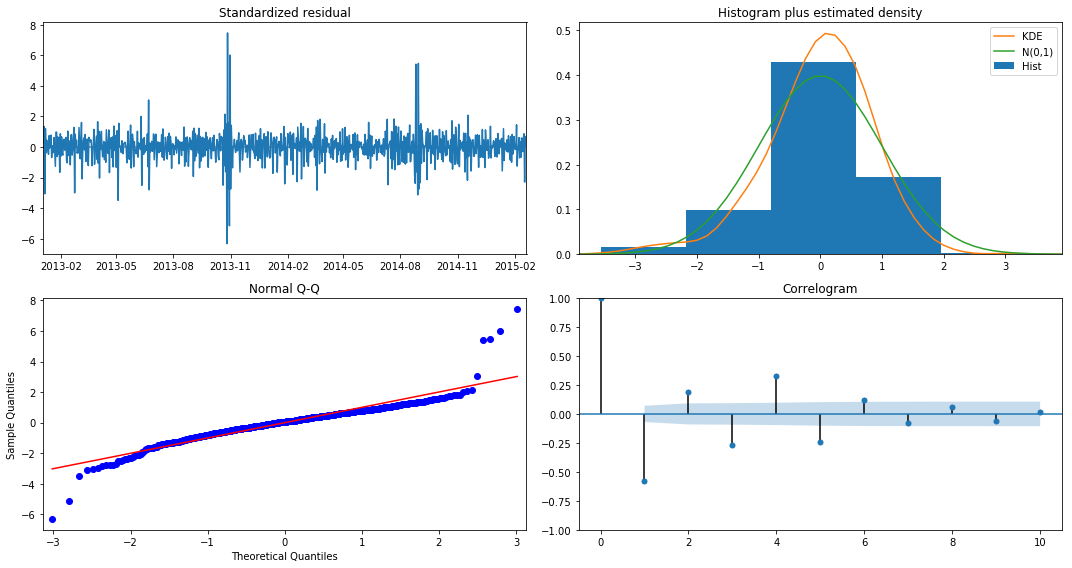
\includegraphics[width=0.99\linewidth]{10_randtrend_res.png}
\endminipage\hfill
\end{figure}
\end{block}

\begin{block}{Локальный линейный тренд с сезонностью}

\begin{figure}[htb]
\minipage{0.49\textwidth}
\begin{gather*}
y_t = \mu_t + \gamma_t + \varepsilon_t,  \varepsilon_t \sim \mathcal{N}(0, \sigma_\varepsilon^2)
\\
\mu_t = \mu_{t-1} + \beta_{t-1} + \eta_t, \eta_t \sim \mathcal{N}(0, \sigma^2_\eta)
\\
\beta_t = \beta_{t-1} + \zeta_t, \zeta_t \sim \mathcal{N}(0, \sigma_\zeta^2)
\\
\mu_1 \sim \mathcal{N}(a_1, P_1) 
\\
\gamma_t = - \sum_{j=1}^{s-1} \gamma_{t+1-j} + \omega_t, \omega_t \sim \mathcal{N}(0, \sigma_\omega^2)
\end{gather*}
\endminipage \hfill
\minipage{0.49\textwidth}
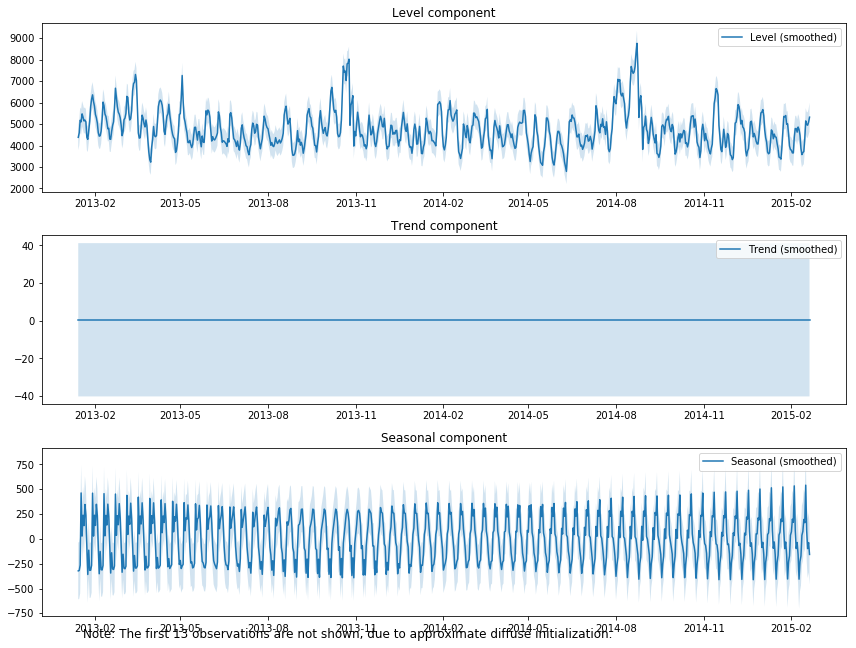
\includegraphics[width=0.99\linewidth]{11_seasonal_dec.png}
\endminipage\hfill
\end{figure}

\begin{figure}[htb]
\minipage{0.49\textwidth}
  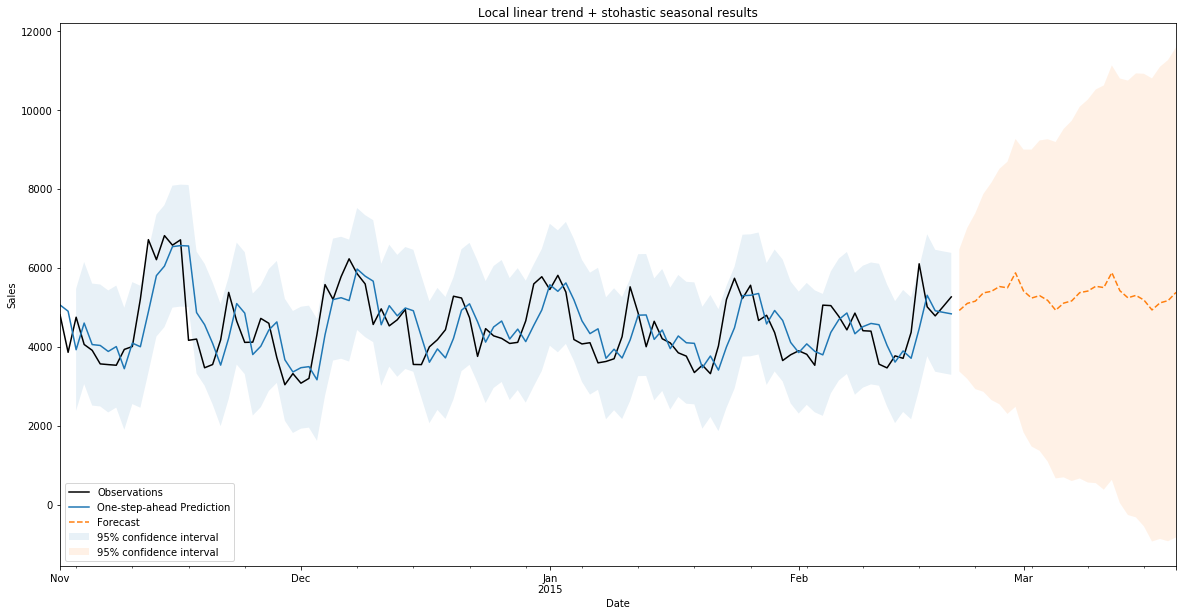
\includegraphics[width=0.99\linewidth]{11_seasonal.png}
\endminipage\hfill
\minipage{0.49\textwidth}
  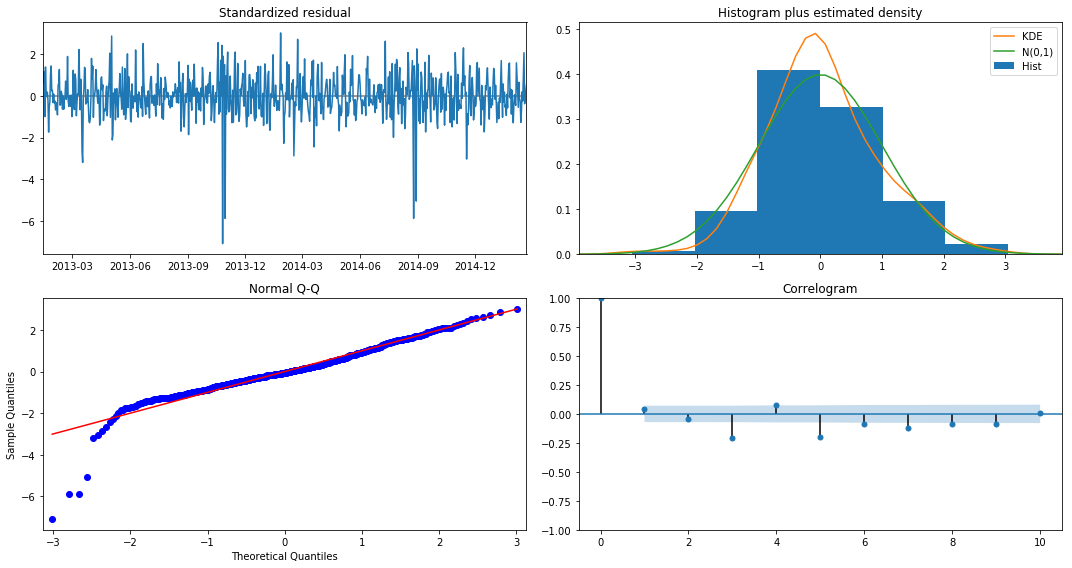
\includegraphics[width=0.99\linewidth]{11_seasonal_res.png}
\endminipage\hfill
\end{figure}

\end{block}

\begin{block}{Локальный линейный тренд с сезонностью и регрессорами}

\begin{figure}[htb]
\minipage{0.49\textwidth}
\begin{gather*}
y_t = \mu_t + \gamma_t + \delta_1^T x_t + \delta_2^T z_t + \varepsilon_t, \varepsilon_t \sim \mathcal{N}(0, \sigma^2_\varepsilon)
\\
\mu_t = \mu_{t-1} + \beta_{t-1} + \eta_t, \eta_t \sim \mathcal{N}(0, \sigma^2_\eta)
\\
\beta_t = \beta_{t-1} + \zeta_t, \zeta_t \sim \mathcal{N}(0, \sigma_\zeta^2)
\\
\mu_1 \sim \mathcal{N}(a_1, P_1) 
\\
\gamma_t = - \sum_{j=1}^{s-1} \gamma_{t+1-j} + \omega_t, \omega_t \sim \mathcal{N}(0, \sigma_\omega^2)
\end{gather*}
\endminipage \hfill
\minipage{0.49\textwidth}
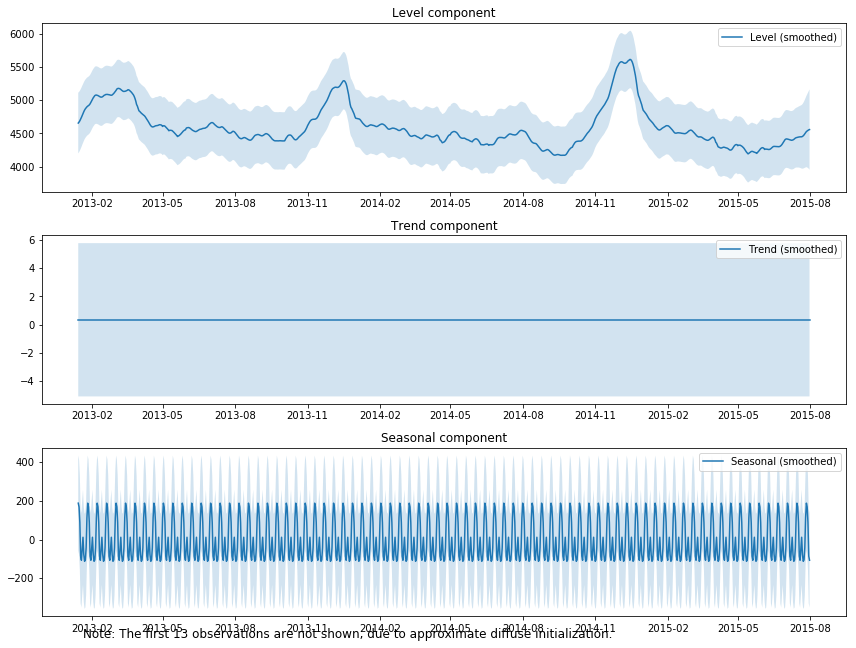
\includegraphics[width=0.99\linewidth]{12_regressors_dec.png}
\endminipage\hfill
\end{figure}

\begin{figure}[htb]
\minipage{0.49\textwidth}
  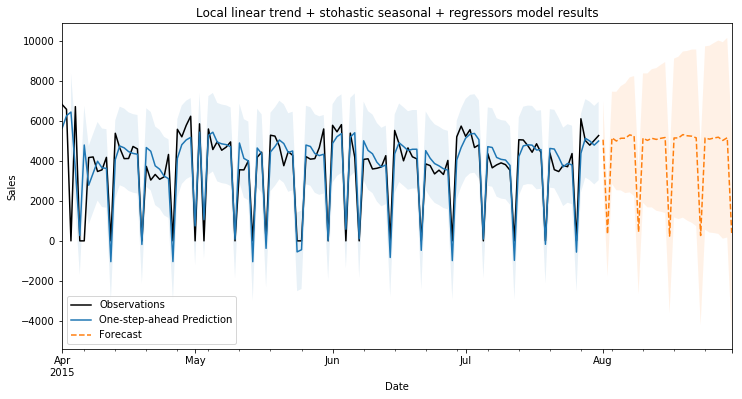
\includegraphics[width=0.99\linewidth]{12_regressors.png}
\endminipage\hfill
\minipage{0.49\textwidth}
  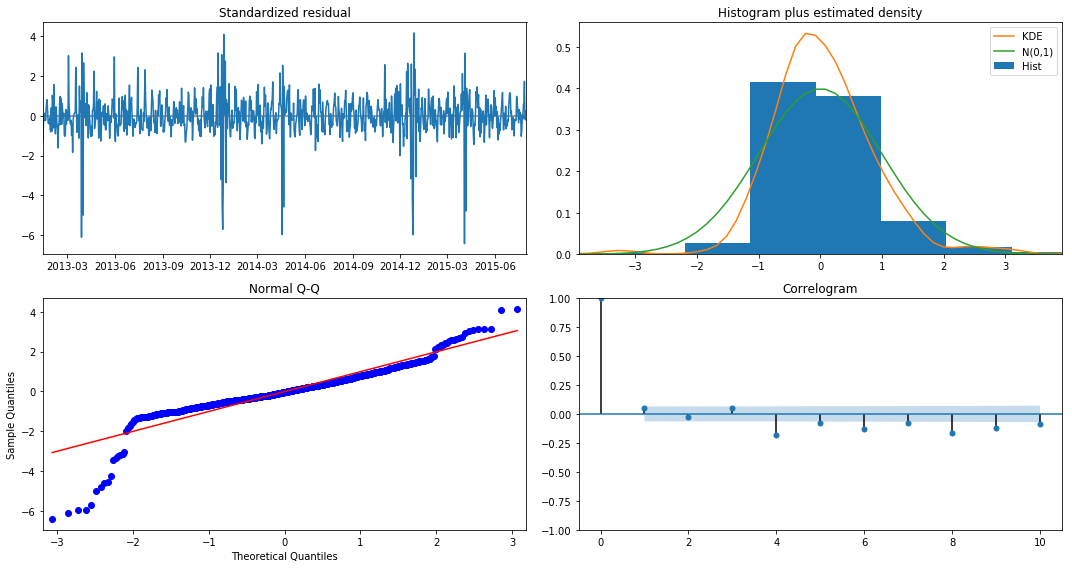
\includegraphics[width=0.99\linewidth]{12_regressors_res.png}
\endminipage\hfill
\end{figure}

\end{block}


\end{column}
\end{columns}



\end{frame}
\end{document}